\subsubsection*{Upload Vulnerabilities}
\addcontentsline{toc}{subsubsection}{Upload Vulnerabilities}
\label{Upload_Vuln}
\T{Getting Started}{
To be able to do this room, we need to configure the hosts file of our device, found under \cd{/etc/hosts}. This file is used for local domain name mapping bypassing DNS, i.e actinge one self as the DNS server or making it unnecessary. This will be especially useful in THM, since the DNS service is not available.\\
Furthermore, it allows name-based Virtual Hosting (vhosting), i.e to serve multiple websites from a single webserver.\\
We need to add \cd{[IP] overwrtite.uploadvulns.thm shell.uploadvulns.thm java.uploadvulns.thm annex.uploadvulns.thm magic.uploadvulns.thm jewel.uploadvulns.thm}
Rembember to adjust the hosts file with every new new machine!
}
\T{Introduction}{
Uploading files to a server is a key part ot the interaction with it, but comes with some dangers attached when not administered properly, ranging from minor inconveniencies to full RCE: an attacker with access to a server might alter content, inject malicious webpages, upload illegal content or leak sensitive information, among other things.\\
In this room we will:
\begin{itemize}
\item Overwrite files
\item Upload and execute shells
\item Bypass Client-Side filtering
\item Bypass Server-Side filtering
\item Fool Content-type validation checks
\end{itemize}
}
\T{General Methodology}{
Enumeration is always a key point of attacks, and web attacks are not an exception.\\
In this case, Gobuster is a great tool to enumerate websites and it subdirectories, to know where to start looking. Its general syntax is:
\cdnl{sudo gobuster dir -u [URL] -w [wordlist]}

When dealing with a website or webserver, Burp Suite also comes in very handy, as it allows us to alter our requests as well as the received responses from the server.\\
As to the general procedure, we will resort to the good old ``Poke it with a stick and see what happens''. In this context, that will mean trying to upload something and seeing what happens or what fails: \\
For the client-side filter we look at the code and try to bypass it.\\
For the Server-side filter we try to find out what the filter is looking for and how to bypass its requirements.
}
\T{Overwriting Existing Files}{
A server containing files should implement some checks before accepting any file upload. In this task we will be focusing on the avoiding of any overwriting of previously existing files.\\
Common ways to avoid this are either a time signature relating the file to its upload time at the beginning or the end of the file, or randomizing the file name completely. On the other hand, one can configure the server to not accept a file with the same name as a previously excisting file, requiring the user to change the name of his file and retry later. \\
This all further plays into the topic of permissions, as websites should not be writeable to web users, hence also not overwriteable.\\
Despite not being a common vulnerability, it is still a good place to start when looking for bugs or in a pentesting environment.\\

In the example we see a picture of a dog, whose name (\cd{images/spaniel.jpg}) we learn by looking at the source code of the site. We download another picture, name it equally and upload it, seeing it overwritten.\\

We do the same by going to the \cd{overwrite.uploadvulns.thm} and try to overwrite an image: 
\QA{
What is the name of the image file which can be overwritten?
}{
In the source code we see the image \cd{images/mountains.jpg}, }
We download an nice mountains picture, rename it to mountains.jpg and upload it to the server.
\QA{
Overwrite the image. What's the flag you receive?
}{
We upload the file and see:\\
Well done -- you overwrote the file!\\
Your flag is: 
\F{THM\{OTBiODQ3YmNjYWZhM2UyMmYzZDNiZjI5\}}
}
}
\T{Remote Code Execution}{
While overwriting images is a nuisance for the administrators of said server or website, it is by no means as harmful as Remote Code Execution, which we will be pursuing in this task.\\
\QA{
Run a Gobuster scan on the website using the syntax from the screenshot above. What directory looks like it might be used for uploads?
}{
We first run a GoBuster scan, and after some trying we arrive at the command 
\cdnl{gobuster -e -u shell.uploadvulns.thm -w /usr/share/wordlists/directory-list-2.3-medium.txt}
Note that the newer \cd{gobuster dir} syntax won't work, as apparently that requires an installation from their GitHub repo.\\
As a result we find the subdirectories \cd{/resources} and \cd{/assets}, and following the example we assume that everything we upload will land in the \cd{/resources} directory. We confirm it by uploading the previous \cd{mountains.jpg} file and navigating later to \cd{http://shell.uploadvulns.thm/resources}, finding our file where we expected it to be.\\
}
\QA{
Get either a web shell or a reverse shell on the machine.
What's the flag in the /var/www/ directory of the server?
}{
As instructed, we download the PentestMonkey PHP reverse shell from \href{https://raw.githubusercontent.com/pentestmonkey/php-reverse-shell/master/php-reverse-shell.php}{here}, substitute the IP address of the php reverse shell for out own tun0 THM IP address. We can leave port 1234 as it is. We then start a netcat listener on our device under \cd{nc -lvnp 1234} and upload the reverse shell to the shell site.\\
After trying to access it, the site hangs and doesn't show any server resources, but we see our reverse shell running. From there on, we only have to print the file \cd{/var/www/flag.txt} and get the flag: 
\F{THM\{YWFhY2U3ZGI4N2QxNmQzZjk0YjgzZDZk\}} 
}
}j
\T{Filtering}{
It is not always the case that we need not to bypass defences in order to upload the files or shells we did in the last tasks, so we will look at the main defence mechanisms implemented to avoid the uploading of malicious files to a server.\\

The underlying concept is the one of filtering, be it on one end or the other of the comunication. Hence, it is divided into client-side and server-side filtering.\\
Client-Side filtering takes place in the user's browser before the file gets uploaded to the server. It has a problem despite the advantage the isolation of the file from the server provides: the filter being on the attacker's side makes it very easy to bypass it, and is considered very insecure. These kind of filters run mostly on JavaScript.\\

Server-Side filtering takes place on the server, historically running PHP despite the more recent tendences of C\#, Node.js, Python and Ruby on Rails raising in importance.\\
With this kind of filtering, we have no way of reading the code or completely deactivating the filter, so we have to submit files that conform to the filter but are not what the filter intended to let through.\\
Some of the first filters we'll see, and the ways to bypass them are:
\begin{itemize}
\item Extension Validation: In theory they are used to identify file types, yet they are actually pretty easy to change and trick, e.g file.type1.type2. Still, Windows uses them to identify file types, so they are relevant despite being failure-prone.\\
Different filter types are either based on blacklists (specifying what is not allowed) or whitelists (specifying the only allowed types, rejecting the rest). 
\item File Type Filtering: More thorough than Extension Validation but working on a similar basis: Identifies the file type and decides if they allow the file to be uploaded or not. In order to do this, there are two types to validate the file type: 
\begin{enumerate}
\item MIME validation: MIME stands for Multipurpose Internet Mail Extension and is a type used as an identifyer for files. It takes its name of the historical origin, firstly identifying files for online mail transfer. \\
The syntax for a MIME type is \cd{<type>/<subtype>}, e.g \cd{image/jpeg}.\\
Since the MIME type is based on the extension of the file, it encounters the same problems as the above Extension Validation.
\item Magic Number Validation: Magic Numbers are the most accurate way of determining the contents of a file and consist of a series of bytes at the beginning of the file stating the ``actual'' file type, e.g every PNG file starts with the bytes \cd{ 89 50 4E 47 0D 0A 1A 0A}. This is the kind of filter Unix systems use to determine the file type. It is still alterable, but with a much greater deal of effort than the other methods.
\end{enumerate}
\item File Length Filtering: In order to save resources on the server some servers only accept files up to a certain size. Note that this is usually not a problem when uploading shells, but it might still be the case that we need to find another shell or alter our previous one to fulfil the requirements.
\item File Name Filtering: As stated before, in order to avoid file replacements on the server, some file name filtering should be in place. This might be a randomized addendum to the original name, a time signature or the refusal of the file if the file name is already present. This also means that we might have to look for our updated file under different name when pentesting the security of a webserver\\
Any file should also be sanitized when uploaded to ensure it doesn't contain potentially disrupting characters such as control characters, e.g`;' or unicode characters, null bytes (\%00) or forward slashes on Linux.
\item File Content Filtering: Better suited systems scan the full contents of every uploaded file to check for any potentially harmful content and eventual spoofing to bypass all other filters, but due to its complexity it is also less broadly implemented.
\end{itemize}

Note that in real-world environments multiple filter layers will be in place, so we'll need to tailor our exploit to bypass all filters at the same time. \\
It is also worth noting that knowing the system we are targeting provides a huge advantage, e.g PHP servers were vulnerable to null-byte exploits until version five, or to the injection of PHP code to exif data of a valid image. \\

Back to the reading comprehension questions on this task: 
\QA{
What is the traditionally predominant server-side scripting language?
}{
PHP
}
\QA{
When validating by file extension, what would you call a list of accepted extensions (whereby the server rejects any extension not in the list)?
}{
Whitelist
}
\QA{
[Research] What MIME type would you expect to see when uploading a CSV file?
}{
A quick search gives us the format we need, namely \cd{text/csv}
}
}
\T{Bypassing Client-Side Filtering}{
Client-Side Filtering is the weakest of the above mentioned filters, and mandatorily the first in place. \\
Recall that it being on our side of the communication, on a machine we control, it is usually very easy to bypass.\\
The most common ways of bypassing it are: 
\begin{enumerate}
\item Turn off JavaScript in the browser: As we discussed before, most Client-Side Servers are JS based, hence if we disable it in our browser, the filters won't work any more. This can also have the downside of stopping the website of working completely if its functionality relies too much on JavaScript. If that is the case, some other filter-bypassing method is preferred.\\
\item Intercept and modify the incoming page: We can intercept the website with Burpsuite as it laods and alter it, taking out the JS filter before it reaches our PC. More on this later. 
\item intercept and modify the file upload: This method works at the file upload step after it has already been accepted by the server as it passed the filter, but correcting the file type afterwards to an executable again.
\item Send the file directly to the upload point: If the filter is on the Client-Side, i.e in the browser, we can bypass it by prescinding of the browser and uploading our file directly using \cd{curl}. Its syntax would look like
\cdnl{curl -X POST -F "submit:<value>" -F "<file-parameter>:$@$<path-to-file>" <site>}
To do this we first intercept a successful upload and see the parameters to be passed onto the above request.
\end{enumerate}
Covering the second method we'll use an image from the THM site to illustrate this kind of filter bypassing:\\
Assuming we have found a website to upload files to, we look at its source code, which might look a bit like this:\\
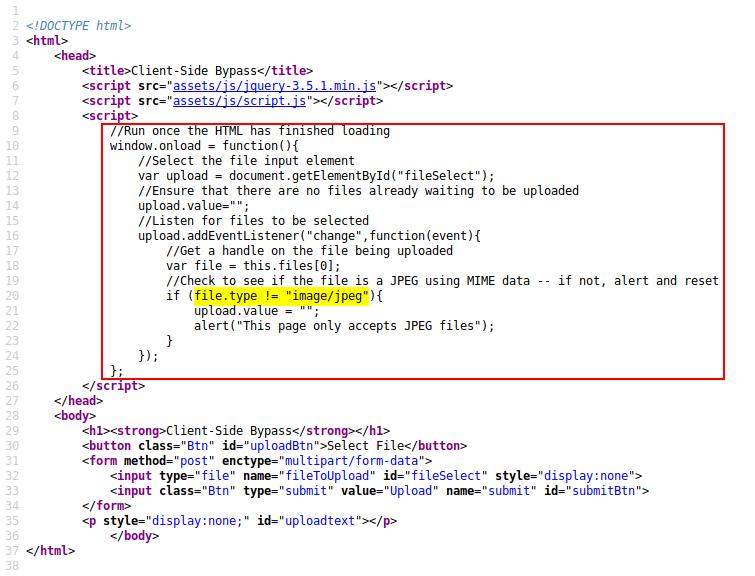
\includegraphics[width=0.8\textwidth]{Complete_Beginner_Path/Web_Hacking_Fundamentals_Room/UploadVulns/images/JSwhitelistCode.png}

There we see taht the filter is a whitelist menat to let only image/jpeg files through. We confirm this by attempting downloads until we see that the only uploaded files are indeed JPEG files.\\
We then start Burp and choose to intercept the response to the page loading request. After forwarding pur request, we can edit the response before it gets to us, hence allowing us to delete the JS script we identified as the whitelist.\\
Once done, we can load the page without any filters and upload any shell we like to the server.\\
Note: Burp will not intercept external JavaScript files the webpage loads unless instructed otherwise under ``Options > Intercept Client Requests > Check File extension does not match:'' and deleting the JS identifier ``$^\wedge$ js\$|''.\\

The other way of bypassing the Client-Side filter is by intercepting and changing our request's MIME type to the accepted MIME, e.g from image/jpeg to text/x-php and the file extension from \cd{shell.jpeg} to \cd{shell.php}, and forwarding it later to the server. That way, the file will mantain its original form and have bypassed the filter.\\

We are now requested to try and put this knowledge into action on our own in the website under \cd{java.uploadvulns.thm}, but a GoBuster Scan is, as always, the best way to start, as the upload directory name will be changing with every new challenge.\\
\QA{
What is the flag in \cd{/var/www}?
}{
We do as advised, set up a Netcat listener on our own Terminal, adapt the PentestMonkey shell to our tun0 THM IP and upload it, in our case to the directory \cd{/images}, assuming the sentence about the randomization was not that true after all.\\
We go to \cd{http://java.uploadvulns.thm} and see that only \cd{.png} files are allowed.\\
We upload such a file and check it lands on the subdirectory \cd{/images}.\\

We then have two possibilities: Either reload the main page and intercept the response, then deleting the lines \cd{<script src="assets/js/client-side-filter.js"></script>}, which we assume to be the filter. As supposed, once disabled, we can upload any shell we want.\\
The other possibility is masquerading our file under the extension \cd{.png} and uploading it, to whose request we see the MIME extension \cd{image/png}. We change this MIME to \cd{text/x-php} and delete the \cd{.png} extension of the masqueraded file.\\

We later set up the Netcat listener on our terminal under port 1234 as before and access the file, gaining RCE. We then see the flag under /var/www/flag.txt and get the flag: 
\F{THM\{NDllZDQxNjJjOTE0YWNhZGY3YjljNmE2\}}
}
}
\T{Bypassing Server-Side Filtering: File Extensions}{
More common and more secure are the Server-Side filters. In this task, we are seeing the code, but (logically) this will never be the case. What we see is that the code looks for the file extension by finding the last period and determining the extension based on the rest of the name string.\\
This code filters \cd{.php} and \cd{.phtml}, but we can to upload our PHP file under another extension, e.g \cd{.php3, .php4, .php5, .php7, .phps, .php-s, .pht, .phar} which would also bypass the filter, but most of them are not recognised as PHP files and hence also not exceuted as such. Note that this is currently the default for Apache2 servers. If luckily for us, the server is out of date, we can attempt each file extension until one works as a recognised PHP file but is not thrown out by the filter. We then upload the ``right'' extension and get our RCE.\\

On the other hand, we can also bypass a (this time obscured) filter by assuming that it only looks for the right extension anywhere in the name. Assuming that \cd{.png} files are allowed, we hope for the file \cd{shell.png.php} to work, still being recognised as a PHP executable.\\

With this at hand, we try to get a reverse shell on \cd{http://annex.uploadvulns.thm}. We first check that \cd{.png} files are accepted by the filter. We further check that PHP files are not allowed when trying to directly upload our shell.\\
After our GoBuster scan is done, we see the directories \cd{/privacy}, where we suspect our files to be, and \cd{/assets}. Trying to see the files, we access \cd{http://annex.uploadvulns.thm/privacy} and see our files with a datestamp added at the beginning, hence changing its name. \\
We now try to bypass the filter by uploading a PHP shell with \cd{.png} in its name, but to no success. \\
We further try to bypass the filter by changing the PHP extension, and after trying \cd{.php, .php3, .php4} without success, we upload a file successfully when having an extension \cd{.php5}. We then go again to the \cd{/privacy} site and run our shell to get the flag under \cd{/var/www/flag.txt}:
\F{THM\{MGEyYzJiYmI3ODIyM2FlNTNkNjZjYjFl\}}
}
\T{Bypassing Server-Side Filtering: Magic Numbers}{
We earlier saw that magic numbers can also be implemented as Server-Side filtering. We can add some characters at the beginning of the file to make the magic numbers of our shell agree with those of the allowed files. This is easiest done by adding a number of characters equal to the length in bytes of the magic number of the \textbf{allowed} file, and then changing them to the desired magic numbers using \cd{hexeditor}.\\

In this case we see a message under \cd{http://magic.uploadvulns.thm} asking us only for GIFs as files to be uploaded.\\
We manage to upload a simple GIF, and running a Gobuster scan we see the subdirectory \cd{/graphics}, where we assume our uploaded GIF to have landed.\\
We check this to be the case calling for the whole path of our file (in our case \cd{/graphics/obiwan.gif}) to circumvent the 403 access forbidden message that arises when trying to access the ``bare'' \cd{/graphics} subdirectory. We edit our PHP shell to make it look like a GIF file by adding to it the magic number \cd{47 49 46 38 39 61}. This is the case for our uploaded GIF, so we check it to be right.\\
We add 6 letters at the top of the PHP shell and edit them later to look like this magic number. After uploading this changed file and setting up our netcat listerner we access our PHP shell and access the flag under \cd{/var/www/flag.txt}:
\F{THM\{MWY5ZGU4NzE0ZDlhNjE1NGM4ZThjZDJh\}}
}
\T{Example Methodology}{
\label{Methodology_WebSite_Audit_Vuln}
Before the last challenge, we use this task as a recapitulation for the general methodology when auditing a website in search of upload attack vulnerabilities in form of the following enumeration: \\
\begin{enumerate}
\item Inspect the website as a whole, be it with Wappalyzer or by hand. Important things to look for are the frameworks and languages the website has been built using. Instead of relying totally on the automated tools, a good way to start is also intercepting the response to any request we make to the website and looking at headers such as \cd{server} and \cd{x-powered-by}. 
We further want to look for attack vetors such as upload pages.
\item If we found an upload page, we inspect it further on our side to bypass any eventual client-side filters. 
\item We attempt an innocent file upload and see how to access the ``unharmful'' file we just uploaded. Main questions when doing so are: \begin{itemize}
\item Can we access it directly in an uploads folder?
\item Is it embedded in a page somewhere?
\item What is the naming scheme of the website?
\end{itemize}
Here the use of Gobuster comes in very handy to find eventual subdirectories where these files may be stored.\\
Especially useful is Gobuster's \cd{-x} switch, used to look for certain extensions when combing over the website and looking for the files with these extensions and names in the provided wordlist. For instance, the switch \cd{-x php, txt, html} appends \cd{.php, .txt, .html} to the names in our wordlist and looks for them. This is especially used when the server changes our file's name.
\item Once we know where and how our files land, we attempt a malicious file upload bypassing any client-side filters we encounter to check for the server-side filters.\\
Either by the provided error messages or by trial and error, we can then tailor our payload to bypass all filters and be executed once it lands on the server.
\end{enumerate}
Depending on the responses from the server, we can assume the kind of server-side filter we are dealing with: 
\begin{itemize}
\item If a totally invalid file extension is allowed (e.g \cd{file.madeupextension} we can assume the filter works based on a blacklist.\\
Else we assume the server is based on a whitelist.
\item If we change the magic number of the unharmful file the server already accepted in the first instance to something more harmful and it gets rejected, we assume the server-side filter is based on a black- or whitelist of magic numbers. 
\item If we change the MIME type of the unharmful file from before to something potentially harmful and it gets rejected, we assume the filter is based on MIME types.
\item When uploading files to the server, there may be a size filter in place as well. Starting small and uploading the same kind of unharmful files until it gets dropped by size we can ascertain the size limit on the server side. 
\end{itemize}
}
\T{Challenge}{
\QA{
Head over to jewel.uploadvulns.thm.\\

Take what you've learned in this room and use it to get a shell on this machine. As per usual, your flag is in /var/www/. Bear in mind that this challenge will be an accumulation of everything you've learnt so far, so there may be multiple filters to bypass. The attached wordlist might help. Also remember that not all webservers have a PHP backend...
}{
After deploying the machine and giving it time to boot, we run a Gobuster scan using the wordlist the task provides, unfortunately without any success. Nonetheless, when running a GoBuster Scan on the site with another wordlist, we see the following subdirectories and response codes: \cd{/content : 301, /modules : 301, /admin: 200, /assets:301}. After looking at the allowed admin site, we see the following text above an entry text field: ``As a reminder: Use this form to activate modules from the modules directory''.\\
Now we have an attack vector: Upload a file to \cd{/modules} and execute it from here.\\

Using Wappalyzer does provide us of the insight of the code the website is written in, namely Node.js. We will then have too look for an exploit for this programming language instead of using our classical Pentest Monkey.\\

Luckily for us, the error messages on upload are very explicit, so we try uploading different images to the server and getting the error message ``Invalid File Format'' for \cd{.jpg, .png and .gif}. When uploading a JPEG-File (which our file uploader identifies by default, we get the message ``File Too Big'' on a file 368kB big. After cropping down the smae file and reducing it to 239 kB we try to upload it and see the message ``File Successfully Uploaded''. So we'll keep that in mind for a moment while we try to ascertain whuch other filters are in place.\\
To see the site, we intercept the response to our site loading request and see the interesting header ``\cd{X-Powered-By: Express}''.\\
When looking at the HTML code intercepted in the Burp proxy, we see what we assume to be the client-side filter: 
\cdnl{<script src="assets/js/upload.js"></script>}
Deleting this line completely prevents us from uploading any files, so we reload the site keeping it in place and look at the details of the file in Firefox's Source Inspector, seeing the full details of the filter:\\
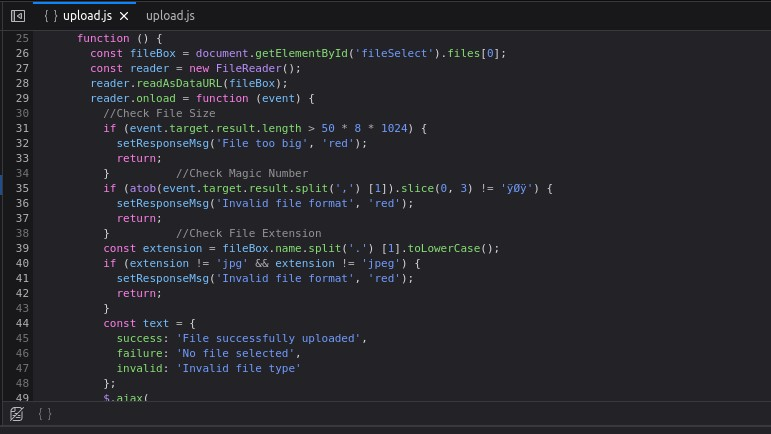
\includegraphics[width=0.95\textwidth]{Complete_Beginner_Path/Web_Hacking_Fundamentals_Room/UploadVulns/Client_side_filter.jpg}
This way, we know what we have to upload:\\
A file smaller than 400 kB whose Magic Number is \cd{FF D8 FF}  and which has as first extension \cd{.jpg} or \cd{.jpeg}.\\
Else, we can disable the filter by allowing Burp to intercept JS requests by deleting the ``$^\wedge$\$js|'' on the Request Interception Rules > File extension Does not match on Burp and deleting the filter on the response to the request to the JS file \cd{upload.js} and we'd the upload our file freely.\\

Now we ``only'' need to know where our innocent file upload lands into, and how to access it:\\
From the site enumeration from Burp as well as our educated guess, we assume the uploaded images to land in th \cd{/contents} subdirectory. We further see all names of the images consisting of three capital letters, e.g \cd{ABH.jpg}. \\
This is when we will resort to the wordlist provided for the task, as a look into it confirms that it is made up of three letter combinations. A Gobuster scan in the form of 
\cdnl{gobuster -e -u jewel.uploadvulns.thm/content -w UploadVulnsWordlist.txt -x jpeg,jpg}
will hopefully give us what we need. \\
We there find the files \cd{ABH.jpg, LKQ.jpg, SAD.jpg, UAD.jpg} as previous jewel images and \cd{TZG.jpg} as our uploaded file. Hence, when we upload the disguised shell, we have to scan again to find out the name the server gave our file and execute it.\\

Summing up, if we don't disable the client-side filter we need to create an executable that: 
\begin{enumerate}
\item has MIME \cd{image/jpeg}.
\item weights less than 400 kB.
\item has .jpeg or .jpg in the name.
\end{enumerate}
We cannot use the reverse shell form the previous tasks, since that one was menat to exploit PHP and now we have a Node.js prgrammed website.\\
We find ready-to-go reverse shells for almost everything under \href{https://swisskyrepo.github.io/InternalAllTheThings/cheatsheets/shell-reverse-cheatsheet/}{Internal All The Things}, so we copy the one for Node.js, write it under a jewelshell.js file after adapting port and tun0 IP and get ready to adjust it to the server-side filters.\\
We then run another Gobuster scan to see which file stands out when compared to the previous one and assume this must be our shell. In our case this appears to be \cd{FBU.jpg}.\\
Once we know which file we have to target, we start a Netcat listener on our terminal and go to the admin site we founf at the beginning, which only executes commands present in the /modules directory. Hence, we can call our script with \cd{../content/FBU.jpg} and see after a short delay that we have a reverse shell. After looking a bit around, we find the file \cd{flag.txt} in the folder above the one we land in and get:
\F{THM\{NzRlYTUwNTIzODMwMWZhMzBiY2JlZWU2\}}
}
Before we end, a short summary of the procedure, step by step: 
\begin{enumerate}
\item Enumerate the site running a gobuster scan.\\
Here we found the subdirectories /content, /modules, /admin and /assets, of which only /admin is freely accessible.
\item Get more information about the site using Wappalyzer.\\
In this case, we used the fact that the webiste is programmed in Node.js.
\item Upload an innocent file to try and follow its path in the server by enumerating the files in the expected subdirectory that can correspond to the adapted name of our innocent file.\\
Here we used the provided namelist to tell the default images from the first scan apart from the name of our image in the second scan.
\item Intercept the source code of the website with Burp, especially the response to the site loading request.\\
If there are some special files, we disable the ignorance of them to inspect them more in detail. \\
In this case, we decided to inspect js files and found the upload.js file with the client-side filter.
\item Disable the client-side filter either with Burp, disabling JS for our browser, or with any other equivalent method.\\
Here we simply deleted the part of this file responsible for the size, MIME and Magic Number filter.
\item We tailor a script or reverse shell for the programming language of the server.\\
In this case we find a Node.js reverse shell in \href{https://swisskyrepo.github.io/InternalAllTheThings/cheatsheets/shell-reverse-cheatsheet/}{Internal All The Things} we adapt to our IP and port. 
\item We try to upload the downloaded shell bypassing server-side filters, e.g magic Numbers, MIME types or file extensions. \\
Here it sufficed to intercept the upload and change the MIME type to image/jpeg.
\item Locate the path to the shell in the server\\
We did this by enumerating (again) the /content directory and locating the new file.
\item Open a listener in our own terminal
\item Execute the shell.\\
We did this this time by going to the /admin site and executing \cd{../content/<name>.jpg}
\item Find the flag or wreak as much havoc as you like.
\end{enumerate}
}